\documentclass[12pt]{article}
\usepackage{pgf}
\usepackage{pgfpages}
\usepackage{hyperref}

\pgfpagesdeclarelayout{boxed}
{
  \edef\pgfpageoptionborder{0pt}
}
{
  \pgfpagesphysicalpageoptions
  {%
    logical pages=1,%
  }
  \pgfpageslogicalpageoptions{1}
  {
    border code=\pgfsetlinewidth{2pt}\pgfstroke,%
    border shrink=\pgfpageoptionborder,%
    resized width=.95\pgfphysicalwidth,%
    resized height=.95\pgfphysicalheight,%
    center=\pgfpoint{.5\pgfphysicalwidth}{.5\pgfphysicalheight}%
  }%
}

\pgfpagesuselayout{boxed}
\usepackage[margin=1.in,includefoot]{geometry}


\usepackage[utf8]{inputenc} % Required for inputting international characters
\usepackage[T1]{fontenc} % Output font encoding for international characters
\usepackage{mathpazo} 
\usepackage{graphicx}
\graphicspath{{images/}}

\begin{document}

\newcommand{\HRule}{\rule{\linewidth}{70mm}}
\center

\textsc{\Huge Blockchain in Healthcare\\ Prevention from Data tampering and Scams}\\[1cm]
\begin{figure}[h]
\centering

\includegraphics[scale=0.9]{nitlogo.png}
\end{figure}


	\begin{minipage}{0.5\textwidth}
		\begin{flushleft}
		\Large
			\underline{ Submitted By:}
			\newline
			
          		Raj Motwani \\
			   Roll No : 21111042 \\
			   Section and Branch -\\Sec ``A'' Biomedical \\
			   Email id : rajmotwani38@gmail.com \\
			   1st Sem
			   
			\end{flushleft}
	\end{minipage}
	~
	\begin{minipage}{0.4\textwidth}
		\begin{flushright}
			\Large
			\underline{ Submitted To :}\\
			
		
			Dr. Saurabh Gupta \\ Department of Biomedical Engineering\\
            NIT Raipur,\\ Chattishgarh,\\
             India, 492013\\
			
			
			
			
		\end{flushright}
	\end{minipage}
	
\newpage
\centering
\section*{\Huge Acknowledgement}
\raggedright
\LARGE I am grateful to Dr. Saurabh Gupta for their proficient supervision of the term project on "Blockchain in Healthcare(Prevention from Data tampering and Scams) ”. I am very thankful to department for their continous guidance and support.\\
	
\raggedleft

\vspace{70mm}

\textbf{Raj Motwani}
\\ \textbf{Roll No:} 21111042


1st semester,
\\ Biomedical Engineering
\\National Institute of Technology,Raipur

\raggedright 
\vspace{110mm}
\section*{ \Huge Abstract }
\Large
\raggedright
The healthcare sector is one of the most important and sensitive industries in the world. The security and privacy of patient data is of utmost importance, and data tampering can have serious consequences.
The use of blockchain technology can help to prevent data tampering and donor scams in the healthcare sector. Blockchain is a distributed database that is tamper-proof and secure. It can be used to store and track patient data, and to verify the authenticity of data.
The use of blockchain technology can help to prevent data tampering and donor scams in the healthcare sector.
For preparing a simple blockchain storage bucket we use solidity programming language and create a smart contract with it (here we are using etherium bockchain).The we will use tools like ganache and truffle to deploy our smartcontract on a test-net before running it on mainnet.And at last using web dev tools like Js,Html,CSS and React.js for creating backend and frontend UI.Also using MySQL for data management.
As Blockchain is immutable so data cannot be manipulated that is already on blockchain.

\section*{ \Huge Introduction }
The lack of accessibility to medical records for both patients and clinicians has long been recognised as a barrier to transparent and efficient healthcare.While electronic health record (EHR) systems help address this issue somewhat, many of these systems are heterogeneous, demonstrate varying success integrating into clinical workflows and exhibit minimal interoperability between platforms. Accordingly, many EHR systems in their present state struggle to deliver fundamental benefits of digital technology such as a streamlined user experience, data sharing capabilities and advanced analytics.This lack of interoperability becomes increasingly challenging as complex patients present to a variety of care providers in different healthcare jurisdictions with various EHR systems. A blockchain-based system is one possible solution conferring several benefits that could be exploited for data federation.That said, blockchain remains a nascent technology and there are key technical, regulatory and institutional barriers that limit its full potential in medicine.
\section*{ \small EHR Systemt based on Blockchain: }
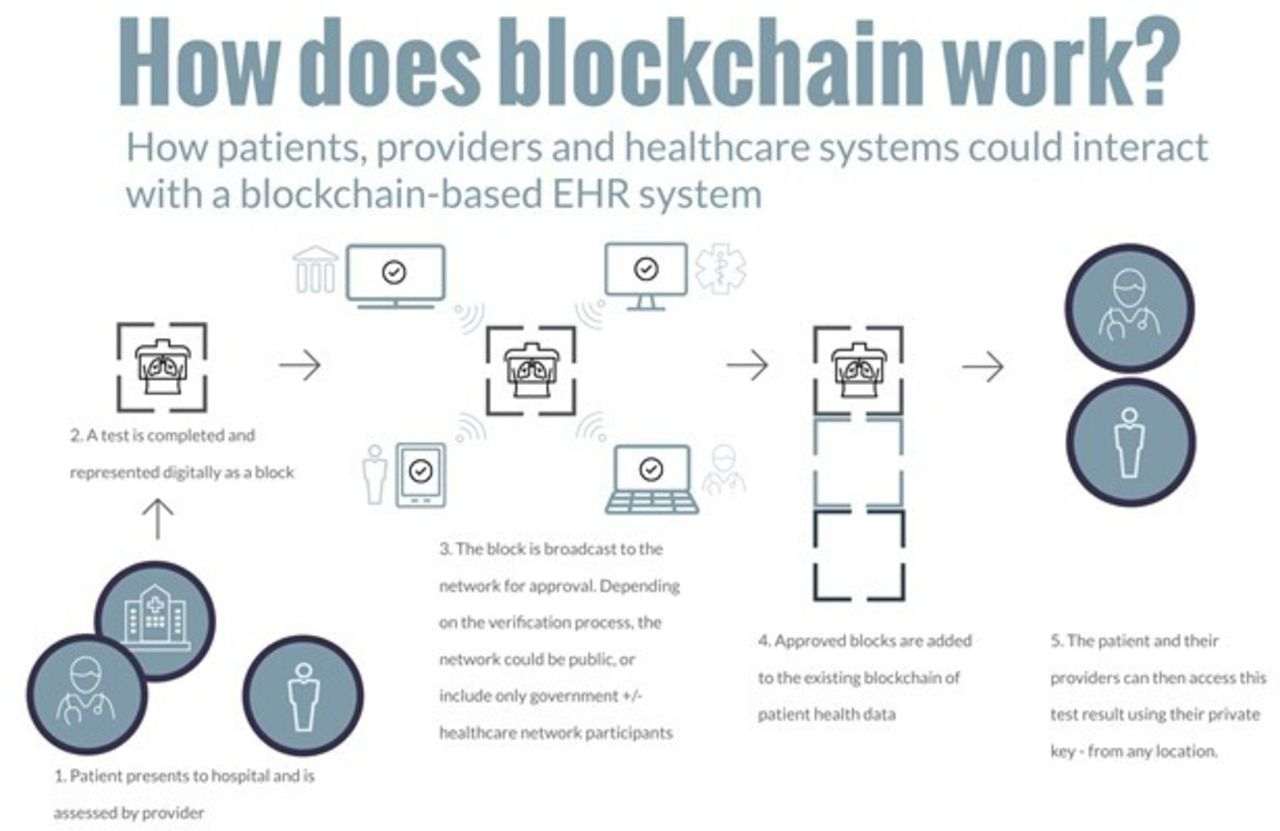
\includegraphics[scale=0.24]{blck.jpg}\\
Blockchain can be used to create a tamper-proof database of patient records. This database can be accessed by doctors and other healthcare professionals, as well as patients themselves. The data in this database can be verified using blockchain technology. This ensures that the data is accurate and secure.
Blockchain can also be used to track donations made to charity organisations. This information can be stored on a blockchain ledger, so that it is secure and tamper-proof. This information can be used to prevent fraudsters from stealing donations from charities.
The use of blockchain technology can help to prevent data tampering and donor scams in the healthcare sector. It can also help to ensure that patient records are accurate and secure, and that donations are tracked and used for the intended purpose. Overall, blockchain is a valuable tool that can be used in the healthcare sector to protect the privacy of patients and donors.\\
\Large \textbf Why it is needed: \\

 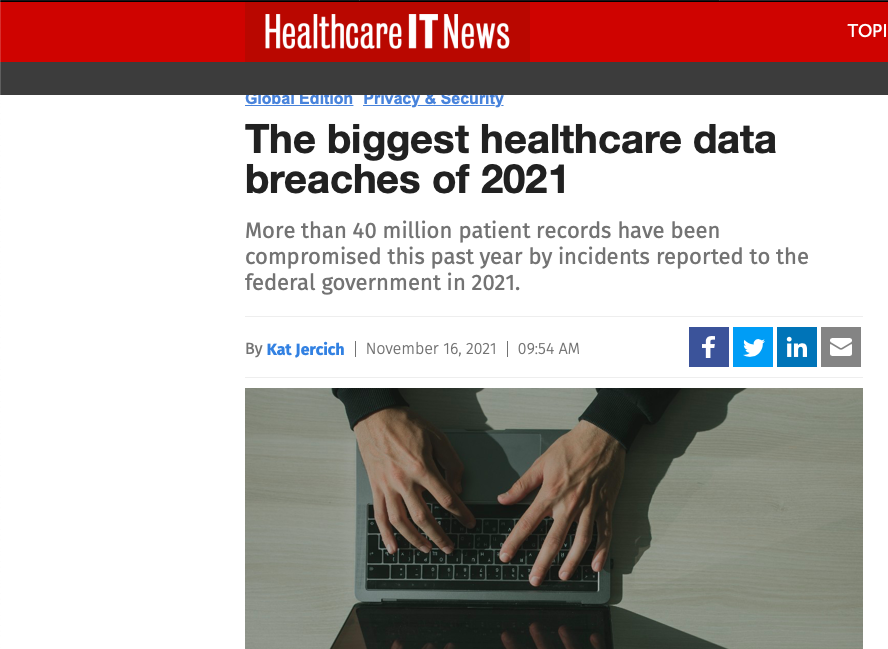
\includegraphics[scale=0.3]{news.png}\\
 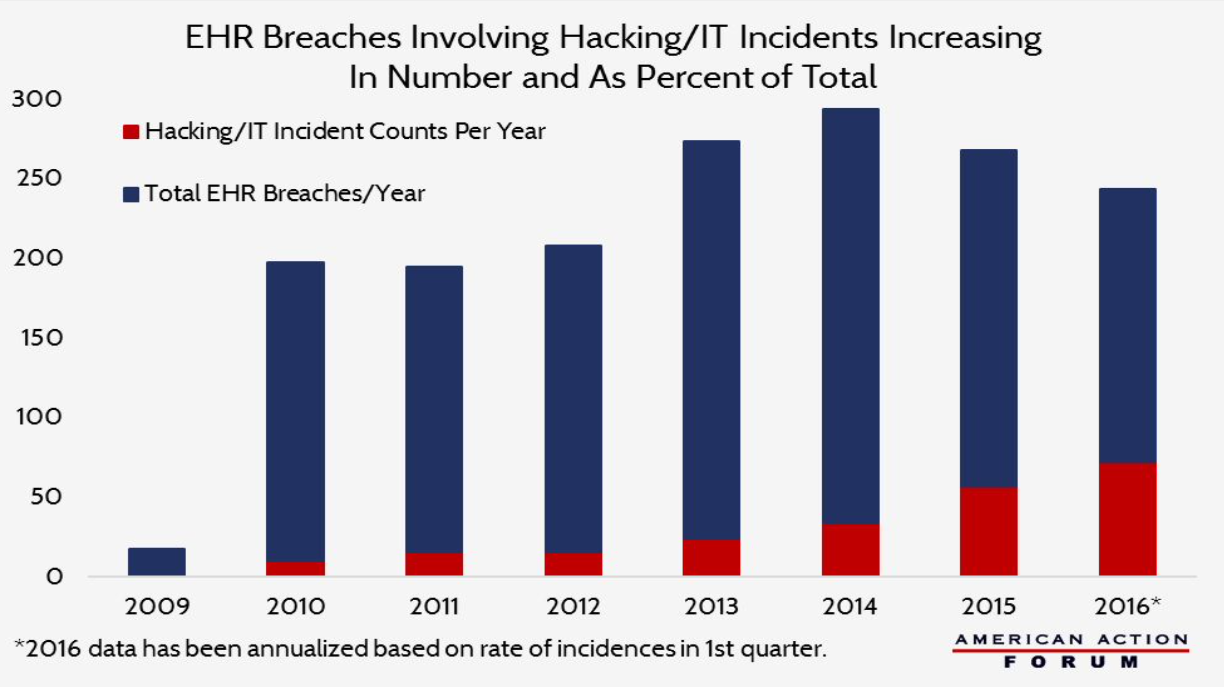
\includegraphics[scale=0.4]{ss2.png}
 \section*{ \Large Sample UI of Portal: }


\normalsize Login Portal:
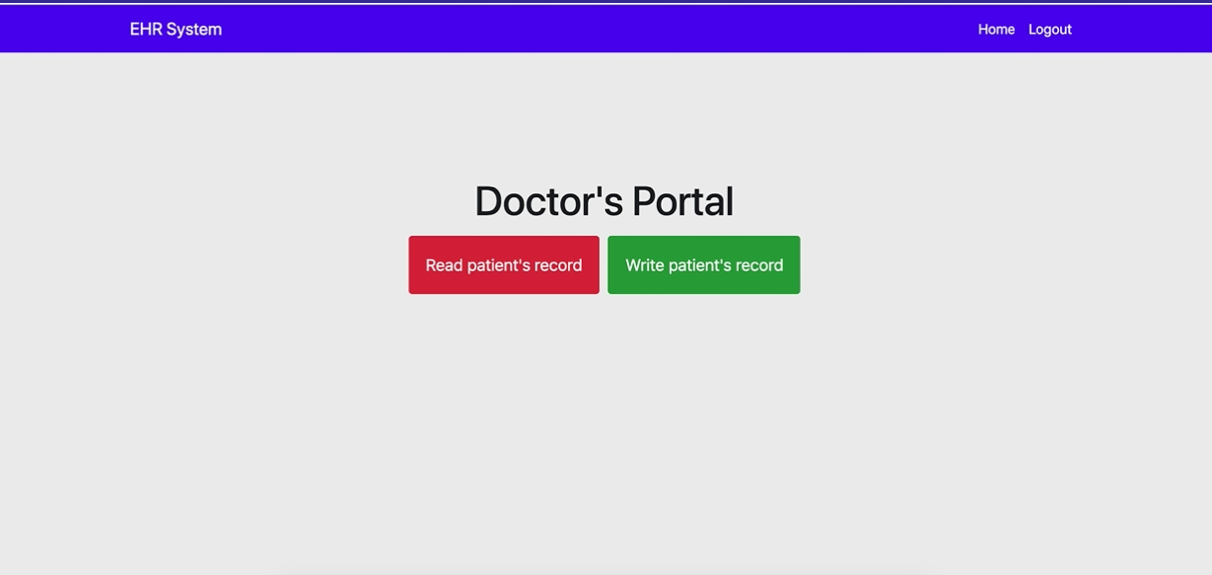
\includegraphics[scale=0.4]{ss4.png}\\
\newpage
Data Entry Portal
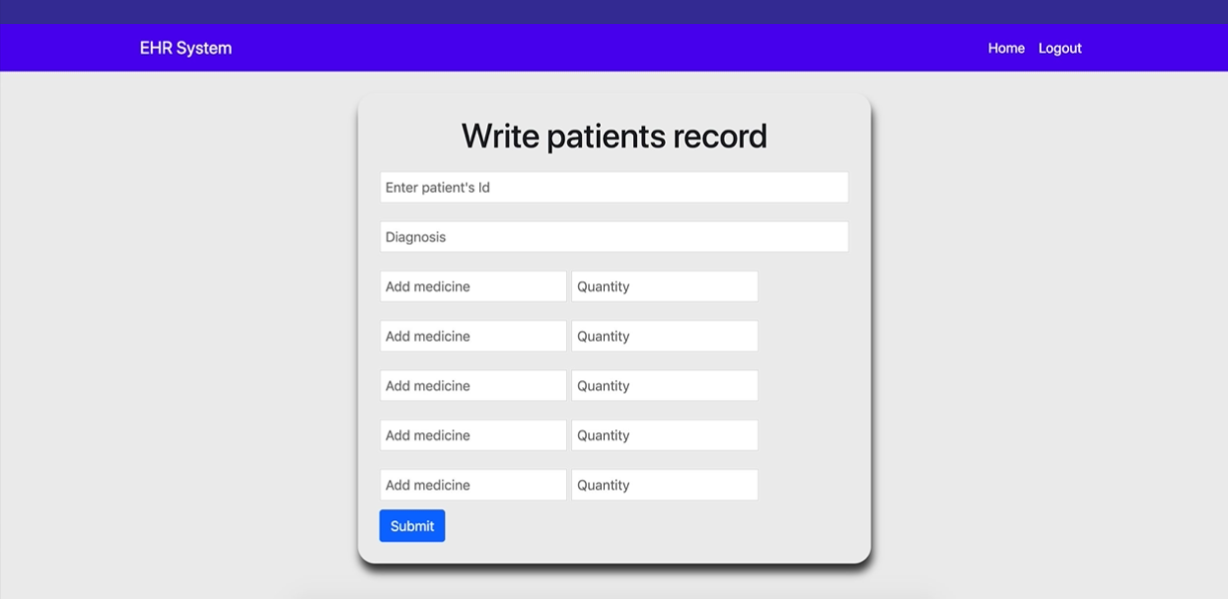
\includegraphics[scale=0.4]{ss3.png}\\
\Large
\section*{\Huge Conclusion: }
With its ability to deflate the current spending bubble, protect patient data and improve overall experience, using blockchain in healthcare may help ease the pain. The technology is already being used to do everything from securely encrypt patient data to manage the outbreak of harmful diseases.
Blockchain has a wide range of applications and uses in healthcare. The ledger technology facilitates the secure transfer of patient medical records, manages the medicine supply chain and helps healthcare researchers unlock genetic code.\\

\vspace{10mm}
\section*{\large How it is working:}
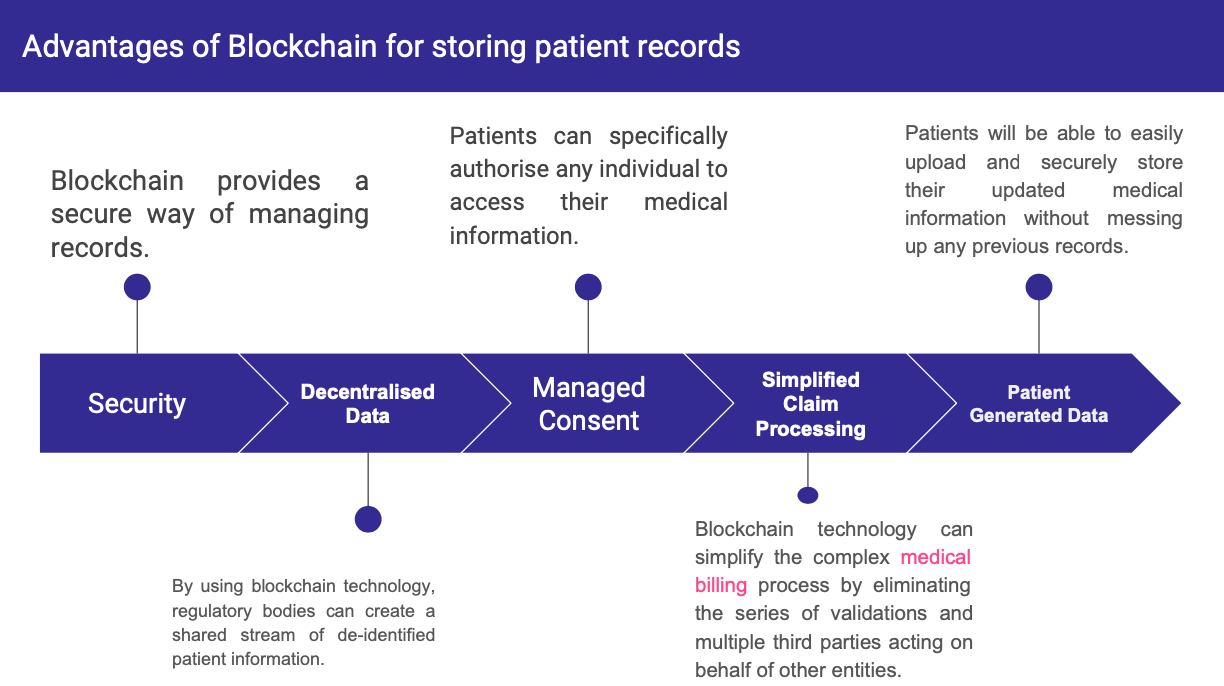
\includegraphics[scale=0.37]{ss1.png}
\section*{\Huge References:}
\normalsize
\url{https://builtin.com/blockchain/blockchain-healthcare-applications-companies}.
\\
\vspace{3mm}
\url{https://github.com/Akshat-Jain/Electronic-Health-Record-System}
\\\vspace{3mm}

\url{https://www.sciencedirect.com/science/article/pii/S266660302100021X}

	
	





 
\end{document}
